% Renamed/adapted from ACM acmart sample.
% Local course report (not an ACM submission).
\documentclass[manuscript,screen]{acmart}

% --- Turn off ACM-specific metadata blocks for a course report ---
\settopmatter{printacmref=false}
\renewcommand\footnotetextcopyrightpermission[1]{}
\pagestyle{plain}

\usepackage{booktabs}
\usepackage{siunitx}
\usepackage{subcaption}
\usepackage{enumitem}

\title{Information Retrieval Final Assignment: Cross-Encoder Re-ranking, Fusion, and Query Expansion}

\author{Mayuresh Khalane}
\affiliation{%
  \institution{Information Retrieval (Course Assignment)}
  \city{Your City}
  \country{Your Country}
}
\email{your.email@university.edu}

\begin{abstract}
This report studies cross-encoder re-ranking for passage retrieval. We fine-tune three cross-encoders on MSMARCO, evaluate them on TREC DL'19 (43 queries) using NDCG@10, Recall@100, and MAP@1000, and provide a reproducible script-based pipeline for run fusion (ranx) and optional query expansion with a local LLM (Ollama).
\end{abstract}

\begin{document}
\maketitle

\section{Introduction}
Neural re-rankers are a standard component of modern retrieval systems: a fast first-stage retriever produces a candidate set (e.g., top-1000), and a more expensive model re-scores these candidates to improve ranking quality. Cross-encoders are strong re-rankers because they jointly encode the query and passage, but they are computationally heavier than bi-encoders.

\subsection{Motivation}
This assignment provides hands-on experience with: (i) fine-tuning cross-encoders on MSMARCO, (ii) evaluating on a standard benchmark (TREC DL'19), and (iii) improving results via rank fusion and (optionally) query expansion.

\section{Background}
\subsection{Cross-encoder re-ranking}
A cross-encoder takes a query--passage pair as input and outputs a relevance score. It is typically used to re-rank a fixed candidate set.

\subsection{Rank fusion}
Fusion combines multiple ranked lists into a single ranking. Methods such as CombSUM, CombMNZ, Borda, and Reciprocal Rank Fusion (RRF) can improve robustness by leveraging complementary strengths of different models.

\subsection{LLM-based query expansion (optional)}
Query expansion aims to rewrite or extend a query with additional terms. Prompting an LLM can generate expansions, and pseudo-relevance feedback (PRF) can supply top-ranked passages as additional context.

\section{Experimental Setup}
\subsection{Datasets}
\begin{itemize}[leftmargin=*]
  \item \textbf{Training:} MSMARCO passage re-ranking.
  \item \textbf{Evaluation:} TREC Deep Learning 2019 (43 queries) with the official candidate set and qrels.
\end{itemize}

\subsection{Models}
We fine-tune the following models for approximately one hour each:
\begin{itemize}[leftmargin=*]
  \item \texttt{cross-encoder/ms-marco-MiniLM-L-2-v2}
  \item \texttt{cross-encoder/ms-marco-TinyBERT-L-2-v2}
  \item \texttt{distilroberta-base}
\end{itemize}

\subsection{Metrics}
We report NDCG@10, Recall@100, and MAP@1000 on TREC DL'19.

\section{Experiments and Results}
\subsection{Task 1: Fine-tuning and Evaluation}
\begin{table}[t]
\centering
\small
\sisetup{round-mode=places,round-precision=4}
\begin{tabular}{l r S S S}
\toprule
Model & Steps ($\approx$1h) & {NDCG@10} & {Recall@100} & {MAP@1000} \\
\midrule
MiniLM-L-2-v2      & 35000 & 0.6721 & 0.4988 & 0.4339 \\
TinyBERT-L-2-v2    & 95000 & 0.6917 & 0.5052 & 0.4553 \\
DistilRoBERTa-base & 11000 & 0.5463 & 0.4733 & 0.3968 \\
\bottomrule
\end{tabular}
\caption{Task 1 results on TREC DL'19 (43 queries) for three fine-tuned cross-encoder re-rankers.}
\label{tab:task1}
\end{table}

\paragraph{Discussion.}
TinyBERT-L-2-v2 achieves the best effectiveness across all metrics, with MiniLM-L-2-v2 close behind. DistilRoBERTa lags behind the MSMARCO-pretrained cross-encoders under the fixed one-hour training budget. One likely reason is that the MS MARCO cross-encoder checkpoints are already specialized for relevance scoring, while DistilRoBERTa starts from a general-purpose LM initialization and may require more optimization time and/or tuning to reach comparable performance.

\begin{figure}[t]
\centering
\begin{subfigure}[b]{0.48\linewidth}
  \centering
  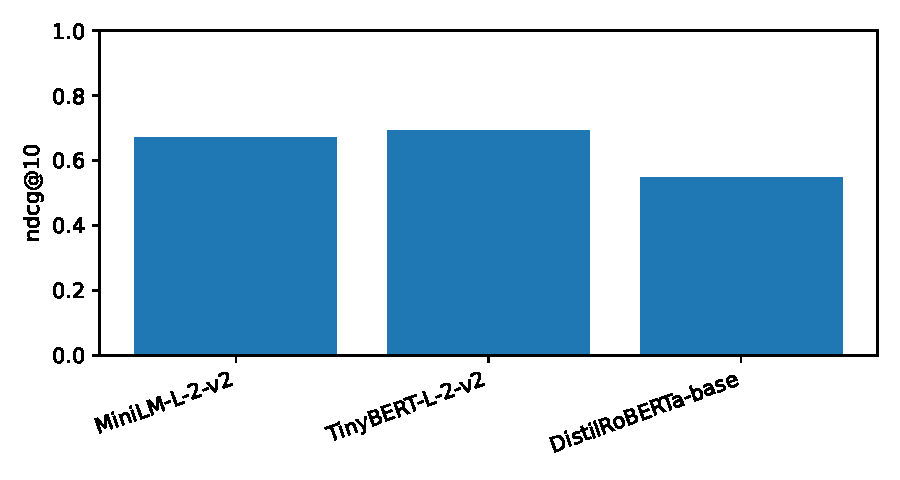
\includegraphics[width=\linewidth]{figures/task1_ndcg@10.pdf}
  \caption{NDCG@10}
\end{subfigure}
\hfill
\begin{subfigure}[b]{0.48\linewidth}
  \centering
  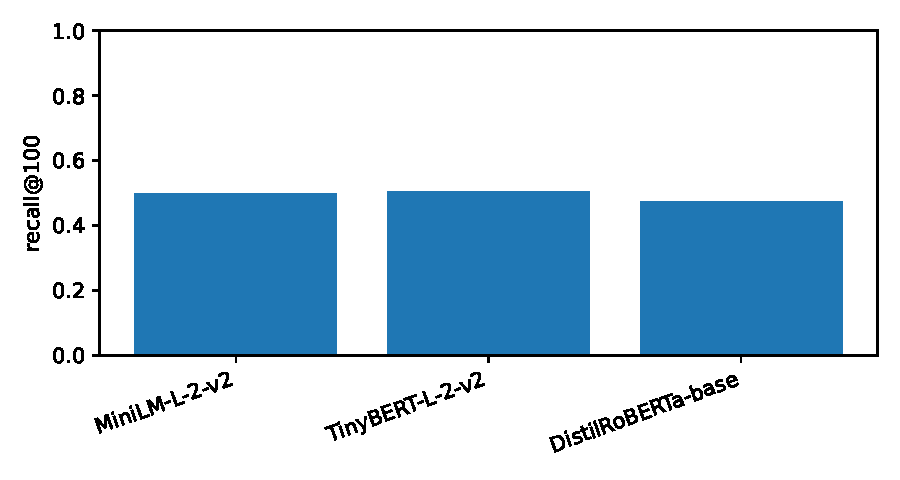
\includegraphics[width=\linewidth]{figures/task1_recall@100.pdf}
  \caption{Recall@100}
\end{subfigure}

\vspace{0.5em}
\begin{subfigure}[b]{0.48\linewidth}
  \centering
  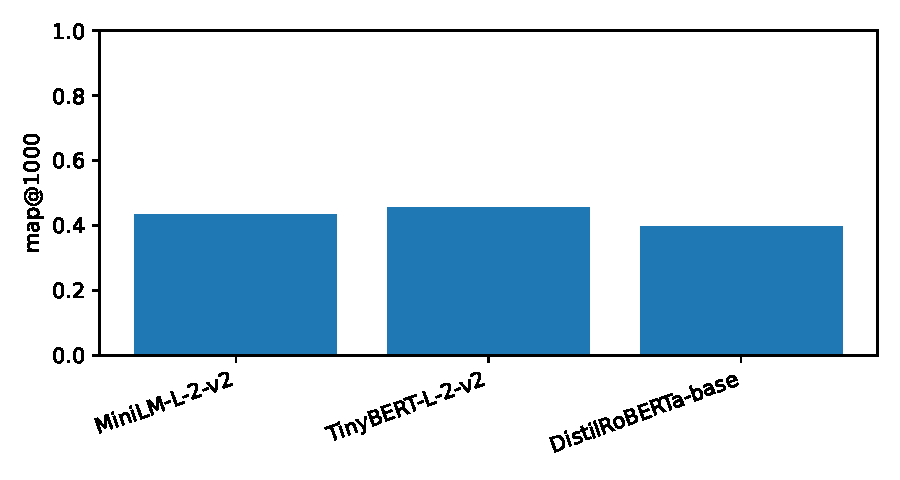
\includegraphics[width=\linewidth]{figures/task1_map@1000.pdf}
  \caption{MAP@1000}
\end{subfigure}
\hfill
\begin{subfigure}[b]{0.48\linewidth}
  \centering
  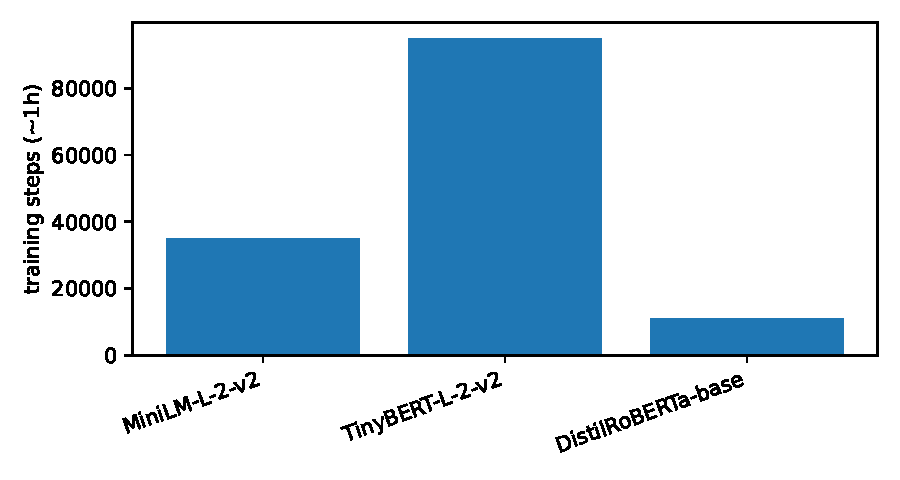
\includegraphics[width=\linewidth]{figures/task1_steps.pdf}
  \caption{Training steps ($\approx$1h)}
\end{subfigure}
\caption{Task 1 summary plots.}
\label{fig:task1_plots}
\end{figure}

\subsection{Task 2: Fusion of Three Runs (Placeholder)}
\textit{To be completed:} Fuse the three Task 1 run files using five fusion methods from \texttt{ranx} and report NDCG@10, Recall@100, and MAP@1000.

\subsection{Task 3: Best Fusion on Two-Run Combinations (Placeholder)}
\textit{To be completed:} Select the best fusion method from Task 2 and apply it to all 2-run combinations.

\subsection{Task 4: LLM Query Expansion (Placeholder, Optional)}
\textit{To be completed:} Generate expanded queries with an LLM prompt and evaluate.

\subsection{Task 5: LLM Query Expansion with PRF (Placeholder, Optional)}
\textit{To be completed:} Add PRF passages into the prompt, evaluate, and compare.

\section{Conclusion}
Under a one-hour fine-tuning budget, the MSMARCO-pretrained cross-encoder checkpoints (TinyBERT-L-2-v2 and MiniLM-L-2-v2) outperform DistilRoBERTa on TREC DL'19. The script-based pipeline supports reproducible evaluation, fusion, and optional query expansion.

\end{document}
